\documentclass{article}

\usepackage{fancyhdr}
\usepackage{extramarks}
\usepackage{amsmath}
\usepackage{amsthm}
\usepackage{amssymb}
\usepackage{amsfonts}
\usepackage{tikz}
\usepackage{physics}
\usepackage[plain]{algorithm}
\usepackage{hyperref}
\usepackage{algpseudocode}

\usetikzlibrary{automata,positioning}

%
% Basic Document Settings
%

\topmargin=-0.45in
\evensidemargin=0in
\oddsidemargin=0in
\textwidth=6.5in
\textheight=9.0in
\headsep=0.25in

\linespread{1.1}

\pagestyle{fancy}
\lhead{\hmwkAuthorName}
\chead{\hmwkClass\ : \hmwkTitle}
\rhead{\firstxmark}
\lfoot{\lastxmark}
\cfoot{\thepage}

\renewcommand\headrulewidth{0.4pt}
\renewcommand\footrulewidth{0.4pt}

\setlength\parindent{0pt}

%
% Create Problem Sections
%

\newcommand{\enterProblemHeader}[1]{
    \nobreak\extramarks{}{Problem \arabic{#1} continued on next page\ldots}\nobreak{}
    \nobreak\extramarks{Problem \arabic{#1} (continued)}{Problem \arabic{#1} continued on next page\ldots}\nobreak{}
}

\newcommand{\exitProblemHeader}[1]{
    \nobreak\extramarks{Problem \arabic{#1} (continued)}{Problem \arabic{#1} continued on next page\ldots}\nobreak{}
    \stepcounter{#1}
    \nobreak\extramarks{Problem \arabic{#1}}{}\nobreak{}
}

\setcounter{secnumdepth}{0}
\newcounter{partCounter}
\newcounter{homeworkProblemCounter}
\setcounter{homeworkProblemCounter}{1}
\nobreak\extramarks{Problem \arabic{homeworkProblemCounter}}{}\nobreak{}

%
% Homework Problem Environment
%
% This environment takes an optional argument. When given, it will adjust the
% problem counter. This is useful for when the problems given for your
% assignment aren't sequential. See the last 3 problems of this template for an
% example.
%
\newenvironment{homeworkProblem}[1][-1]{
    \ifnum#1>0
        \setcounter{homeworkProblemCounter}{#1}
    \fi
    \section{Problem \arabic{homeworkProblemCounter}}
    \setcounter{partCounter}{1}
    \enterProblemHeader{homeworkProblemCounter}
}{
    \exitProblemHeader{homeworkProblemCounter}
}

%
% Homework Details
%   - Title
%   - Due date
%   - Class
%   - Section/Time
%   - Instructor
%   - Author
%

\newcommand{\hmwkTitle}{Assignment\ \#1}
\newcommand{\hmwkDueDate}{Due on 2nd September, 2018}
\newcommand{\hmwkClass}{Fluid Mechanics}
\newcommand{\hmwkClassTime}{}
\newcommand{\hmwkClassInstructor}{}
\newcommand{\hmwkAuthorName}{\textbf{Aditya Vijaykumar}}

%
% Title Page
%

\title{
    %\vspace{2in}
    \textmd{\textbf{\hmwkClass:\ \hmwkTitle}}\\
    \normalsize\vspace{0.1in}\small{\hmwkDueDate\ }\\
%    \vspace{3in}
}

\author{\hmwkAuthorName}
\date{}

\renewcommand{\part}[1]{\textbf{\large Part \Alph{partCounter}}\stepcounter{partCounter}\\}

%
% Various Helper Commands
%

% Useful for algorithms
\newcommand{\alg}[1]{\textsc{\bfseries \footnotesize #1}}

% For derivatives
\newcommand{\deriv}[1]{\frac{\mathrm{d}}{\mathrm{d}x} (#1)}

% For partial derivatives
\newcommand{\pderiv}[2]{\frac{\partial}{\partial #1} (#2)}

% Integral dx
\newcommand{\dx}{\mathrm{d}x}

% Alias for the Solution section header
\newcommand{\solution}{\textbf{\large Solution}}

% Probability commands: Expectation, Variance, Covariance, Bias
\newcommand{\E}{\mathrm{E}}
\newcommand{\Var}{\mathrm{Var}}
\newcommand{\Cov}{\mathrm{Cov}}
\newcommand{\Bias}{\mathrm{Bias}}

\begin{document}

\maketitle

%\pagebreak

\begin{homeworkProblem}
    The \textit{Knudsen Number} is given by,
    $$\text{Kn} = \frac{\lambda}{L} = \frac{k_B T}{\sqrt{2} \pi d^2 p L}$$
    where $L$ is the characteristic length scale, and $T$ and $p$ are the temperature and pressure respectively.
    
    We can take some approximations for the the variations of $T$ and $p$, but we note that data for the variation of $T$ and $p$ is also available publicly \url{http://www.hyvac.com/tech_support/atmosphere%20vs%20pressure%202.htm}.
    We import that data and use it to do our calculations. We also assume some standard values for all the other parameters.
    
    \begin{figure}[!h]
    	\centering
    	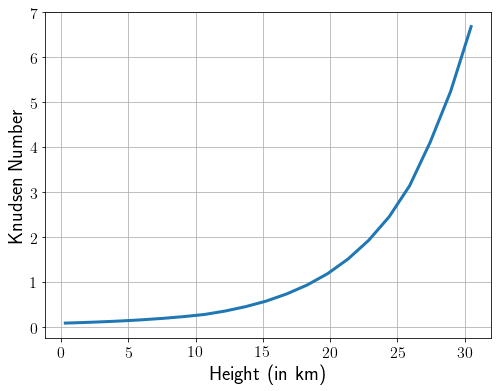
\includegraphics[scale=0.45]{knudsen.png}
    \end{figure}
    
    \end{homeworkProblem}

\begin{homeworkProblem}
	$$\dv{C}{\eta} = \kappa \exp({\frac{-\eta^2}{4D}})$$ where $\eta = x/\sqrt{t}$. 
	Performing the indefinite integral and substituting for $\eta$, one gets,
	$$ C(\eta) = \sqrt{D\pi} \kappa \ \text{erf}\left(\frac{\eta}{2\sqrt{D}}\right) + \alpha = \sqrt{D\pi} \kappa \ \text{erf}\left(\frac{x}{2\sqrt{D}\sqrt{t}}\right) + \alpha$$
	where $\alpha$ is some integration constant. We now go ahead and impose boundary conditions
	\begin{itemize}
		\item The concentration at the flower $(x=0)$ is assumed to be a constant $C_0$ at all times. As erf$(0) = 0$, $\alpha=C_0$
		\item At $t=0$, any $x$ would have zero concentration. As erf$(x \rightarrow \infty) = 1$, We get the condition that $\sqrt{D\pi} \kappa + C_0 = 0$ ie. $\kappa = -C_0/\sqrt{D \pi}$
	\end{itemize}
	
	Therefore, the final solution is,
	$$C(x,t) = C_0\ \left[1 - \text{erf}\left(\frac{x}{2\sqrt{D}\sqrt{t}}\right)\right]$$
	
	
	The function is plotted below for different $t$ using standard value of diffusivity $D \approx 10^{-5} $ $m^2/s$,
	\begin{figure}[!h]
		\centering
		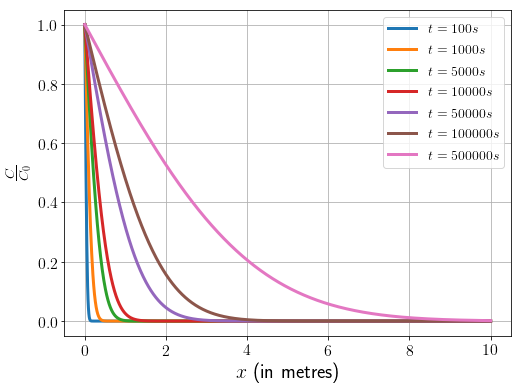
\includegraphics[scale=0.45]{q2.png}
	\end{figure}
\end{homeworkProblem}

\begin{homeworkProblem}
	\textbf{Part (a)}\\
	The continuity equation $(\div{\va{v}}=0)$ in cylindrical coordinates is given by,
	$$\frac{1}{\rho} \pdv{v_\rho}{\rho} + \frac{1}{\rho}\pdv{v_\theta}{\theta} + \pdv{v_z}{z} = 0$$
	
	For flows symmetric about the $\phi$ direction, this can be written as,
	$$\frac{1}{\rho} \pdv{v_\rho}{\rho} + \pdv{v_z}{z} = 0$$
	
	The stream function $\psi$ should be such that,
	$$d \psi = \pdv{\psi}{\rho} d\rho + \pdv{\psi}{z} d z = M d\rho + N d z \implies \pdv{M}{z} = \pdv{N}{\rho}$$
	
	Comparing the forms of the last two equations, one can infer,
	$$M = \pdv{\psi}{\rho} = \rho v_z \text{ and } N = \pdv{\psi}{z} = \rho v_\rho $$
	
	Therefore, the stream function $\psi$ is given by,
	$$\psi = \int \rho v_z d\rho + \int \rho v_\rho d z$$
	
	The streamlines for a cone are plotted in the figure below.
	\begin{figure}[!h]
		\centering
		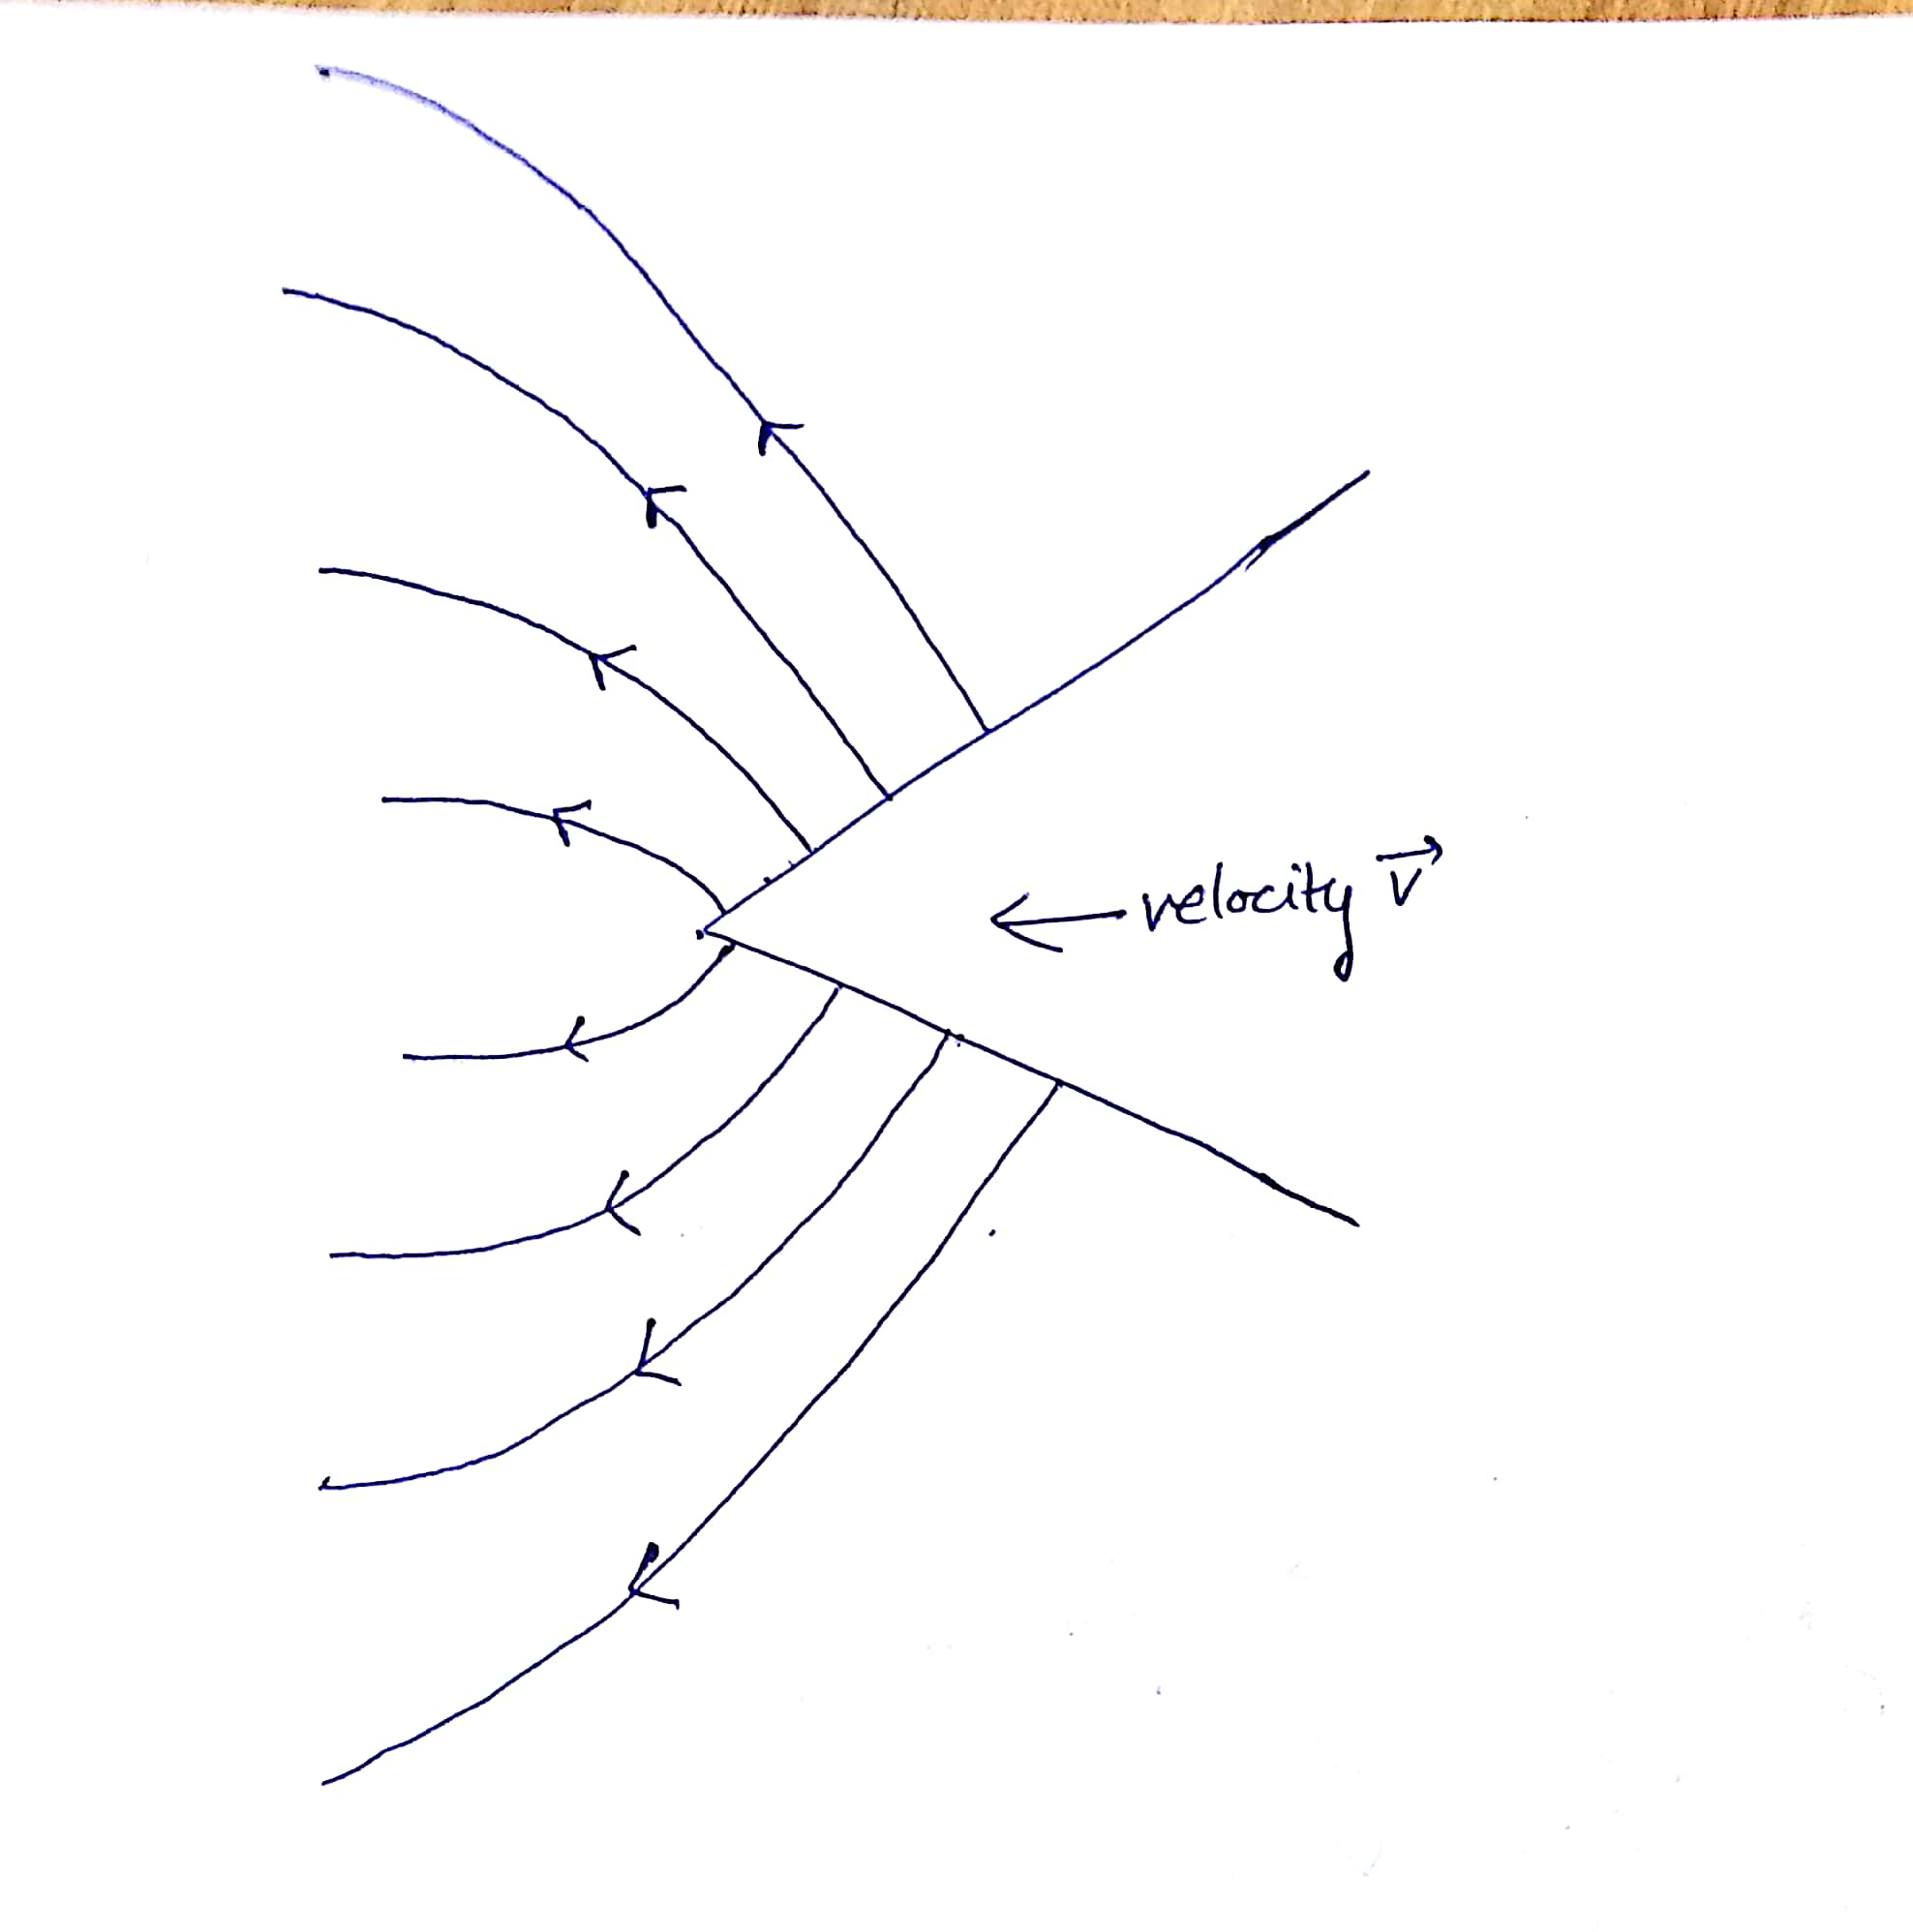
\includegraphics[scale=0.1]{stream.jpg}
		\caption{Flow past moving cone, assuming slip}
	\end{figure}
	\\
	
	\textbf{Part (b)}\\
	The velocity fields at the respective locations of the stream functions as shown in the figure will be $v_1 = \curl{\va{\psi_1}}$ and $v_2 = \curl{\va{\psi_2}}$, where $\va{\psi_1} = (0,0,\psi_1)$ and $\va{\psi_2} = (0,0,\psi_2)$. The streamlines for this flow will meet somewhere in between (because there cannot be two directions of velocity at a single point). For example, such a flow can be generated by two moving infinite plates inclined at an acute angle, and having the no-slip boundary condition.
\end{homeworkProblem}

\begin{homeworkProblem}
	$$\grad{u} = e_{ij} + \Omega_{ij}$$
	We can do the above decomposition of $\grad{u}$ into a symmetric and antisymmetric tensor. \textbf{$\Omega_{ij}$ represents pure rotation}. The symmetric part can be written and the divergence of some $\phi$.
	
	Let the principle axes in the problem be $x$, $y$ and $z$ (different from the coordinate axes). For some constants $a,b,c$, $\phi$ can be written as (in three dimensions),
	\begin{flalign*}
	\phi &= \frac{1}{2}(ax^2 + by^2 + cz^2)\\
	&= \frac{1}{2}\left[\frac{a+b+c}{3}(x^2+y^2+z^2) +\frac{2a - b - c}{3} x^2 + \frac{2b - a - c}{3} y^2 + \frac{2c - b - a}{3} z^2 \right]\\
	&= \frac{1}{2}\left[\alpha(x^2+y^2+z^2) + \alpha_1 x^2 + \alpha_2 y^2 + \alpha_3 z^2 \right]
	\end{flalign*}
	
	We note that $\alpha_1+\alpha_2+\alpha_3=0$. Then,
	\begin{flalign*}
	\phi &= \frac{1}{2}\left[\alpha(x^2+y^2+z^2) + \alpha_1 x^2 + \alpha_2 y^2  -(\alpha_1 + \alpha_2) z^2 \right]\\
	&= \frac{1}{2}\left[\alpha(x^2+y^2+z^2) + \alpha_1 (x^2-z^2) + \alpha_2( y^2-z^2)\right]
	\end{flalign*}
	We see that the first term is symmetric in the coordinates, and hence we remark that it is the pure expansion/contraction term. Similarly, the other two terms are antisymmetric under exchange of coordinates, hence they are pure strain terms. One can make a rotation of coordinates such that $$x^2 - y^2 \rightarrow xy \text{ and } y^2 - z^2 \rightarrow yz$$
	
	One can now make the interpretation of the last two terms as shear strain terms in the rotated coordinates. \textbf{So, we have successfully decomposed the $e_{ij}$ into shear strain $+$ pure expansion/contraction.}
\end{homeworkProblem}
\end{document}
